% Report identifiers
% They are unique alphanumeric designations that may identify the responsible
% organization, the report series/collection and the individual report (i.e.
% Rapporti ISTISAN 05/2 stands for a report of the series Rapporti ISTISAN
% produced in the year 2005 and it is the second report of the year).

% ISSN/ISBN and other codes
% ISSN is the International Standard Serial Number that is assigned on request
% by the ISSN Authority (www.issn.org) for reports that are produced in a
% series; the ISBN is the International Standard Book Number that is assigned
% on request by the ISBN Authority to each single issue (www.isbn.org). The
% report may also have other codes, such as DOI (Digital Object Identifier),
% which may be obtained on request by each authority. More than one code may
% appear in a report.

% Place and date of publication
% It is important to include the place and date of publication, both for
% bibliographic identification and priority concerns. This information may
% appear in the title page or in the back of the title page.

% This document has been modified from its original version by Kathryn Huff
% Acknowledgement of the original version is below.
%
%%%%%%%%%%%%%%%%%%%%%%%%%%%%%%%%%%%%%%%%%
% Academic Title Page
% LaTeX Template
% Version 2.0 (17/7/17)
%
% This template was downloaded from:
% http://www.LaTeXTemplates.com
%
% Original author:
% WikiBooks (LaTeX - Title Creation) with modifications by:
% Vel (vel@latextemplates.com)
%
% License:
% CC BY-NC-SA 3.0 (http://creativecommons.org/licenses/by-nc-sa/3.0/)
%
% Instructions for using this template:
% This title page is capable of being compiled as is. This is not useful for
% including it in another document. To do this, you have two options:
%
% 1) Copy/paste everything between \begin{document} and \end{document}
% starting at \begin{titlepage} and paste this into another LaTeX file where you
% want your title page.
% OR
% 2) Remove everything outside the \begin{titlepage} and \end{titlepage}, rename
% this file and move it to the same directory as the LaTeX file you wish to add it to.
% Then add \input{./<new filename>.tex} to your LaTeX file where you want your
% title page.
%
%%%%%%%%%%%%%%%%%%%%%%%%%%%%%%%%%%%%%%%%%

%----------------------------------------------------------------------------------------
%    PACKAGES AND OTHER DOCUMENT CONFIGURATIONS
%----------------------------------------------------------------------------------------

\documentclass[11pt]{article}

\usepackage[utf8]{inputenc} % Required for inputting international characters
\usepackage[T1]{fontenc} % Output font encoding for international characters
\usepackage{lscape}
\usepackage{mathpazo} % Palatino font
\usepackage{graphicx} % For the logo
\usepackage{subcaption}
\usepackage{float} % Put figures exactly where we need them
% hyperref usually has to go last
\usepackage[hidelinks]{hyperref}
% but glossaries behaves best if after hyperref
\usepackage[acronym,toc]{glossaries}
\include{acros}
\makeglossaries

\begin{document}

%----------------------------------------------------------------------------------------
%    TITLE PAGE
%----------------------------------------------------------------------------------------

\begin{titlepage} % Suppresses displaying the page number on the title page and the subsequent page counts as page 1
    \newcommand{\HRule}{\rule{\linewidth}{0.5mm}} % Defines a new command for horizontal lines, change thickness here

    \center % Centre everything on the page

    %------------------------------------------------
    %    Title
    %------------------------------------------------
    \HRule
    \vspace{0.2cm}
     \begin{minipage}{0.4\textwidth}
	     
\includegraphics[width=\textwidth]{./figures/arfc-logo.png}
        \end{minipage}%
        \begin{minipage}{0.6\textwidth}
        {\begin{flushright}\huge\bfseries UIUC Data Report
                           \end{flushright}}
        {\begin{flushright}\large\textit{Summary of Data for the University of Illinois}\end{flushright}}
        \end{minipage}

    \vspace{0.2cm}
    \HRule
    \vspace{0.5cm}

    %------------------------------------------------
    %    Author(s)
    %------------------------------------------------
       \begin{minipage}{0.4\textwidth}
               \begin{flushleft}
                       \large
                       \textit{Prepared for:}\\
                       \textsc{NEUP Project}\\ %
                        \textsc{Contract} NN-NNNN\\ %
                \end{flushleft}
       \end{minipage}
       ~
       \begin{minipage}{0.4\textwidth}
               \begin{flushright}
                       \large
                       \textit{Prepared by:}\\
                       Samuel \textsc{Dotson} %
                       \vspace{4mm}\\
                       \textit{Principal Investigator:}\\ %
                       Prof. Caleb \textsc{Brooks} % Supervisor's name
               \end{flushright}
    \end{minipage}

    % If you don't want a supervisor, uncomment the two lines below and comment the code above
    %{\large\textit{Author}}\\
    %John \textsc{Smith} % Your name

    %------------------------------------------------
    %    Report Number
    %------------------------------------------------
    \vspace{1cm}
    \textsc{\LARGE\bfseries UIUC-ARFC-2021-00} % Replace YYYY with the year, NN with report index
    \vspace{0.5cm}

    %------------------------------------------------
    %    Date
    %------------------------------------------------

    \vspace{0.5cm} % Position the date further down the remaining page
    {\large February 17, 2021} % January 1, 3000
    % Use the date of actual publication, change the \today to a set date if you want to be precise
    \vspace{0.5cm}

%------------------------------------------------
    %    Headings
    %------------------------------------------------

    \textsc{\LARGE Advanced Reactors and Fuel Cycles}\\[0.25cm] % Research Group

    \textsc{\large Dept. of Nuclear, Plasma, \& Radiological Engineering}\\% Department

    \textsc{\large University of Illiois at Urbana-Champaign}\\ % University



    %------------------------------------------------
    %    Logo
    %------------------------------------------------

    \vspace{0.5cm}
    
\includegraphics[width=0.8\textwidth]{./figures/illinois.eps}\\[1cm] % Include a department/university logo - this will require the graphicx package

    %----------------------------------------------------------------------------------------

    %------------------------------------------------
    %   Funding
    %------------------------------------------------
    % For this section, either use \vfill to fill the space
    % or insert funding acknowledgement
    \textit{Funding Acknowledgement}

\end{titlepage}
%----------------------------------------------------------------------------------------
%\pagebreak
\section*{Introduction}
	Micro-reactors have the potential to be a transformative distributed energy technology that can revolutionize America's energy infrastructure.
	This project seeks to quantify the opportunities and challenges of operating micro-rectors in populated, decentralized power generation environments, and the potential for deployment in established micro-grids with diverse power generation sources.
	The University of Illinois at Urbana-Champaign (UIUC) campus is a good model system for this analysis due to its diverse power generation portfolio and various heating, cooling, and electrical systems.
	UIUC Facilities and Services (F\&S) records generation and consumption data for all of these systems. We have been working with F\&S to obtain data that will inform our system models. Table \ref{tab:datasummary} summarizes all of the data the NEUP team can access. This report gives a brief overview of our data with examples and use cases.


\section{Campus Data}
	The University of Illinois at Urbana-Champaign (UIUC) has a vast amount of
data that can be used to understand patterns and trends at a deep level. There are three main sectors of data from UIUC: electricity data, steam data, and chilled water data.  

	\subsection{Electricity data}
		Electricity data from UIUC comprises of electricity demand and electricity generation. 
		\subsubsection{Campus Electricity Demand}
			Campus electricity demand comprises of electricity demand of all buildings, systems, and utilities.

			
		\subsubsection{Petascale Computing Facility Electricity Demand}
		The National Petascale Computing Facility (NPCF) is a large supercom
			\begin{figure}[H]
			  \centering
			  \includegraphics[width=0.8\textwidth]{./figures/npcf_elec_peaks_labeled.pdf}
			  %\caption{}
			  \label{fig:typstm}
			\end{figure}

		\subsubsection{Abbott Electricity generation}
			Abbott Power plant generates electricity for campus.
		\subsubsection{UIUC Solar Farm 1.0 Electricity generation}
			Solar Farm 1.0 generates electricity for campus.
	
		\subsubsection{Railsplitter Wind Farm Electricity generation}
			UIUC has a PPA with Railsplitte Wind Farm, purchasing 8\% of the electricity the windfarm produces.
	
	\subsection{Steam data}
		UIUC uses central steam for heating.
		\subsubsection{Abbott Low Pressure Steam}
			Low pressure steam is used for\ldots
		\subsubsection{Abbott High Pressure Steam}
			High pressure steam is used for \ldots

	\subsection{Chilled water data}
		UIUC has a chilled water loop and storage tank used for cooling.
		\subsubsection{Campus Chilled Water}
			
		\subsubsection{Petascale Computing Facility Chilled Water}
			NPCF used chilled water for cooling components. NPCF also has three cooling towers to chill its own water during the colder months of the year.
\section{Off-campus Data}
	In addition to the campus data provided by F\&S, we also use local weather data to better inform our model.
	\subsection{Willard Weather Data}
		
	\subsection{Lincoln Weather Data}

	\subsection{CU Weather Data}
	
\section{Synthetic Data}
	The energy system has been further characterized by determining \textit{typical years}
	on campus. These typical years were generated by identifying the typical month --  ``typical" is defined as the closest to a mean value -- for each month of the
	year and combining them to form a typical year. This task was performed using
	the \texttt{RAVEN} tool from INL. Figure \ref{fig:typstm} shows the typical year
	of steam, Figure \ref{fig:typelc} shows the typical year of electricity demand,
	Figure \ref{fig:typwind} shows the typical year of wind power delivered to UIUC, and Figure \ref{fig:typsol} shows the typical year of solar power
	delivered to the campus. These typical years are useful for generating synthetic
	data, also with the \texttt{RAVEN} tool, that can be used for energy system
	optimization with \texttt{Modelica} \cite{epiney_report_2017, baker_optimal_2018}. Figure \ref{fig:synelc} demonstrates this capability.

	\begin{figure}[H]
	  \centering
	  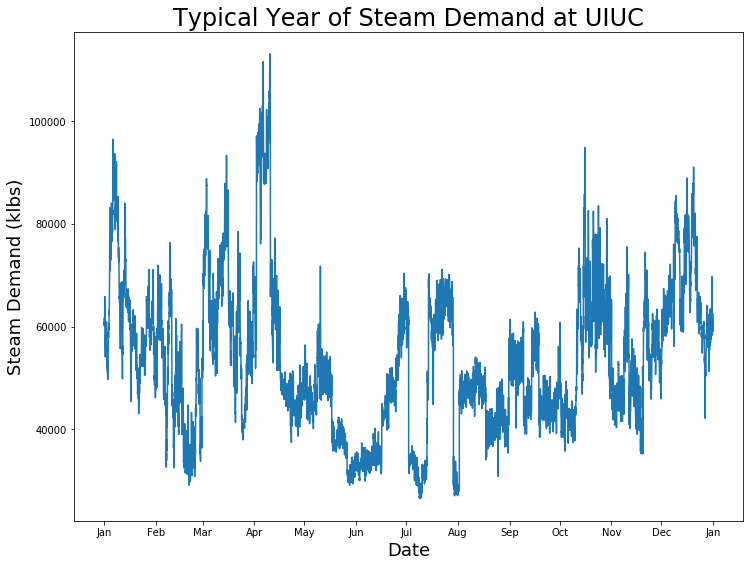
\includegraphics[width=0.8\textwidth]{./figures/typicalsteam.png}
	  \caption{A typical year of hourly steam demand on the UIUC campus}
	  \label{fig:typstm}
	\end{figure}

	\begin{figure}[H]
	  \centering
	  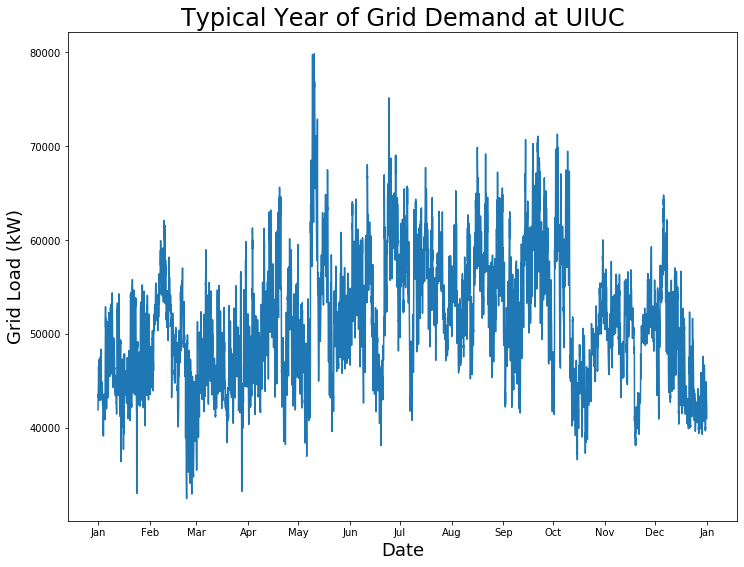
\includegraphics[width=0.8\textwidth]{./figures/typicaldemand.png}
	  \caption{A typical year of hourly electricity demand on the UIUC campus}
	  \label{fig:typelc}
	\end{figure}

	\begin{figure}[H]
	  \centering
	  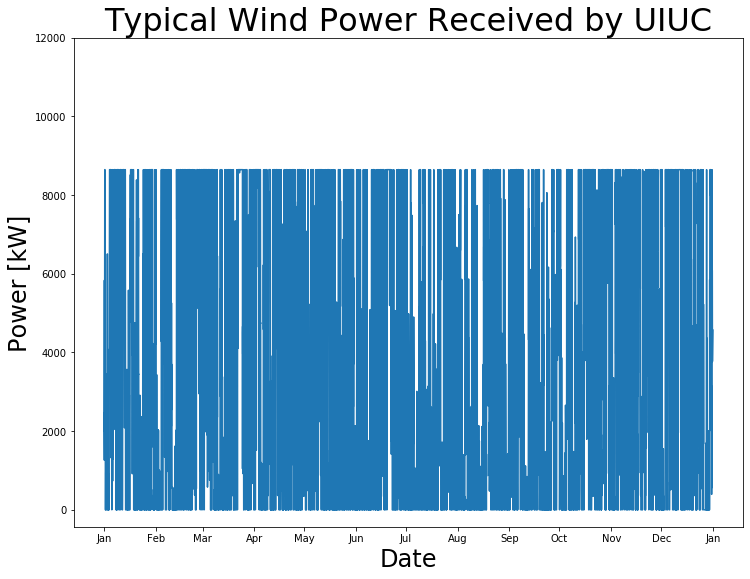
\includegraphics[width=0.8\textwidth]{./figures/typicalwind.png}
	  \caption{A typical year of hourly wind energy supplied to the UIUC campus}
	  \label{fig:typwind}
	\end{figure}

	\begin{figure}[H]
	  \centering
	  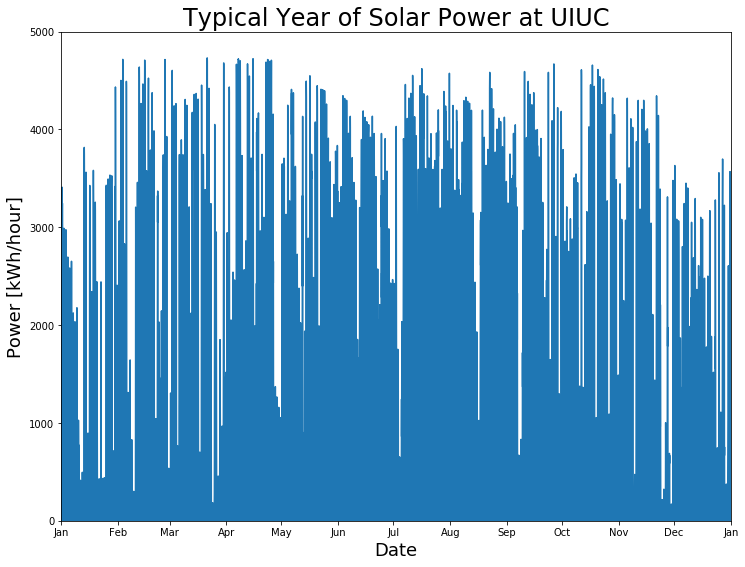
\includegraphics[width=0.8\textwidth]{./figures/typicalsolar.png}
	  \caption{A typical year of hourly solar energy supplied to the UIUC campus}
	  \label{fig:typsol}
	\end{figure}


	\begin{figure}[H]
	  \centering
	  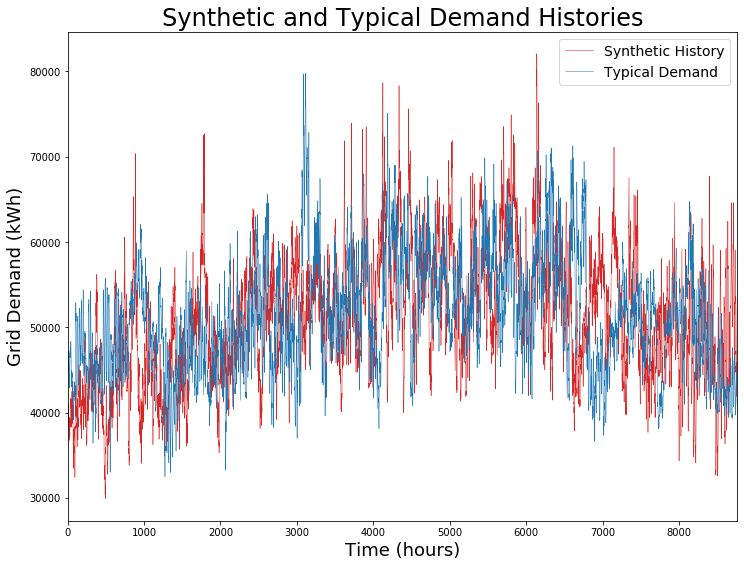
\includegraphics[width=0.8\textwidth]{./figures/syntypdemand.png}
	  \caption{A typical year of hourly electricity demand on the UIUC campus}
	  \label{fig:synelc}
	\end{figure}

\section{Other Data}
	There is more to the UIUC campus energy system than steam and electricity. UIUC
	also has a significant vehicle fleet. Analyzing this data allows us to determine
	the demand for gasoline equivalent energy on campus. This demand may be replaced
	by either electric or hydrogen powered vehicles in the future. Figure
	\ref{fig:fueldemand} shows the demand for three different fuel types on the UIUC
	campus.

	\begin{figure}[H]
	  \centering
	  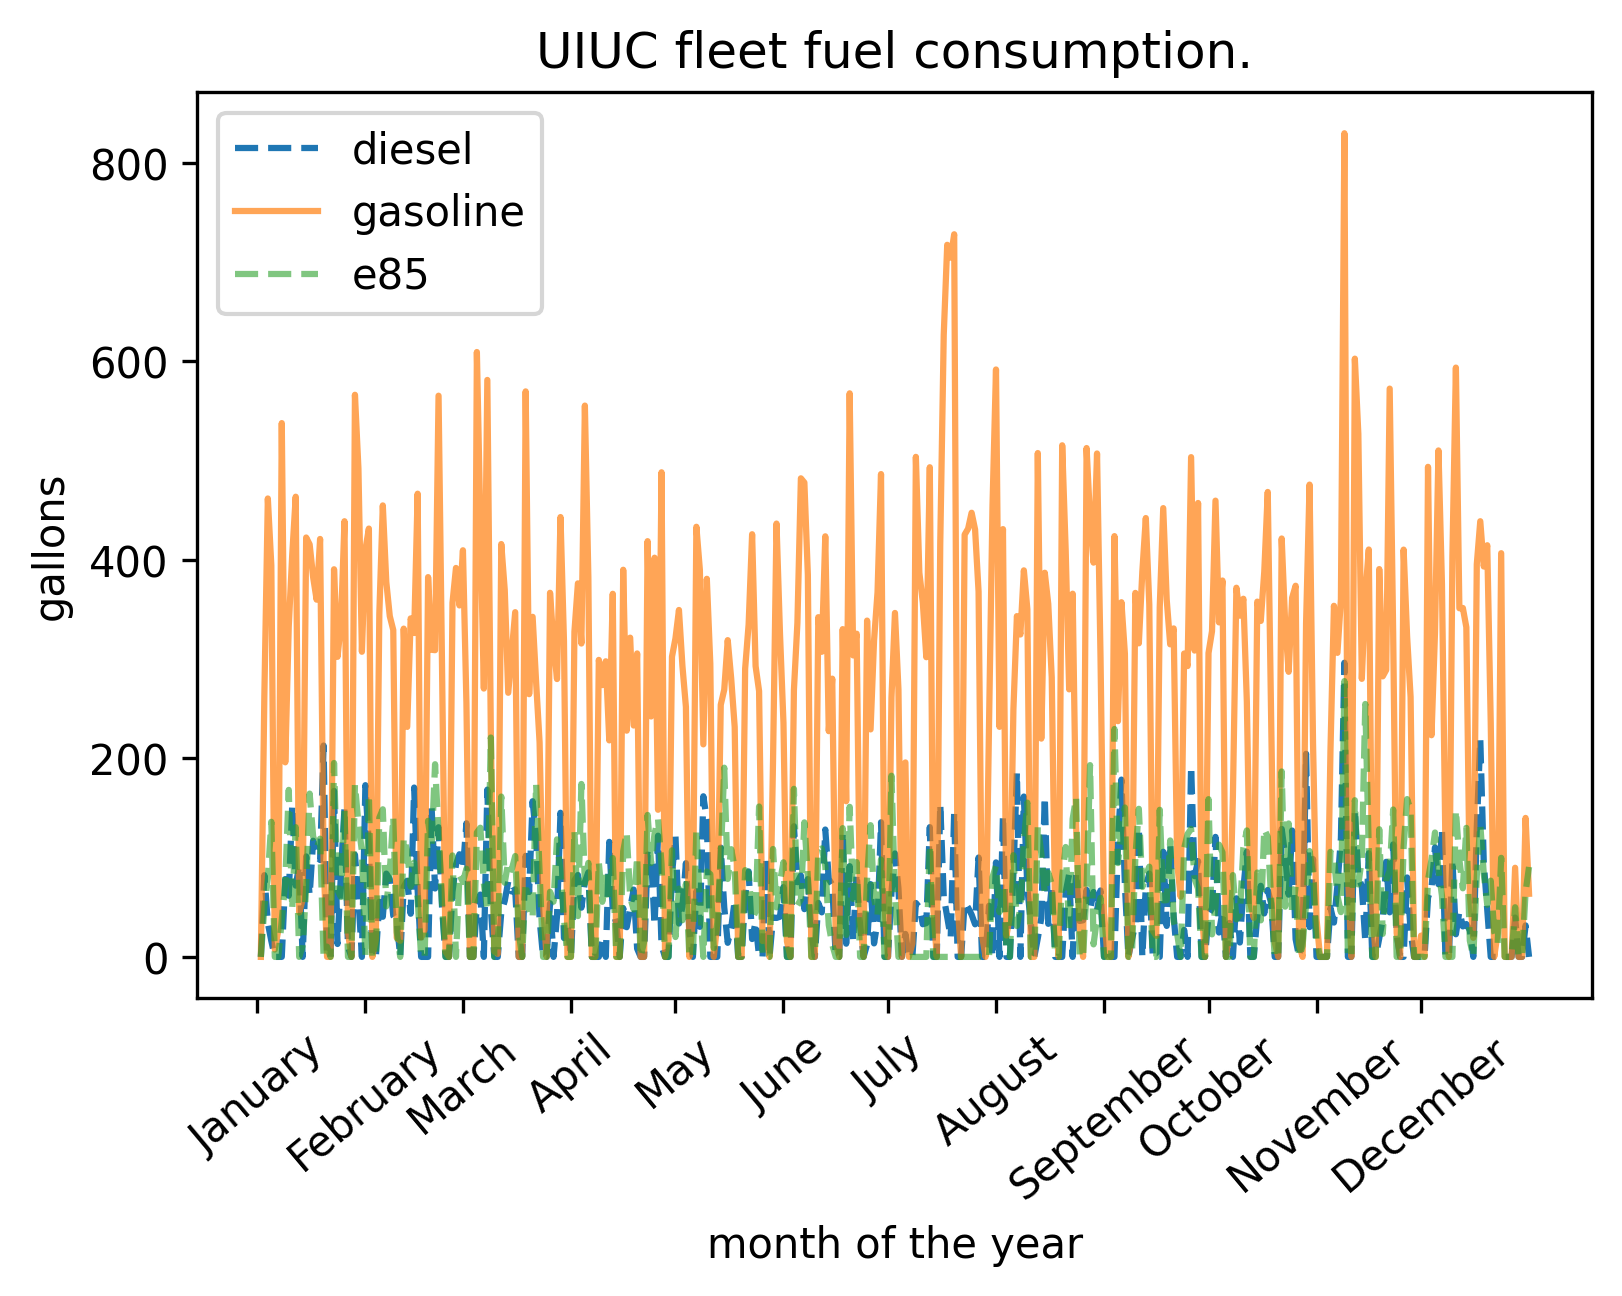
\includegraphics[width=\textwidth]{./figures/uiuc_fueldemand.png}
	  \caption{The demand for three types of fuel for one year on the UIUC campus.}
	  \label{fig:fueldemand}
	\end{figure}

\section{Data processing}
	Before the data from UIUC Facilities and Services (F\&S) can be used, it must
	be checked for data flagged as ``unreliable'' or otherwise incorrect values.
	The first step in this data processing is shown in Figure \ref{fig:unreliable}
	\begin{figure}[H]
	  \centering
	  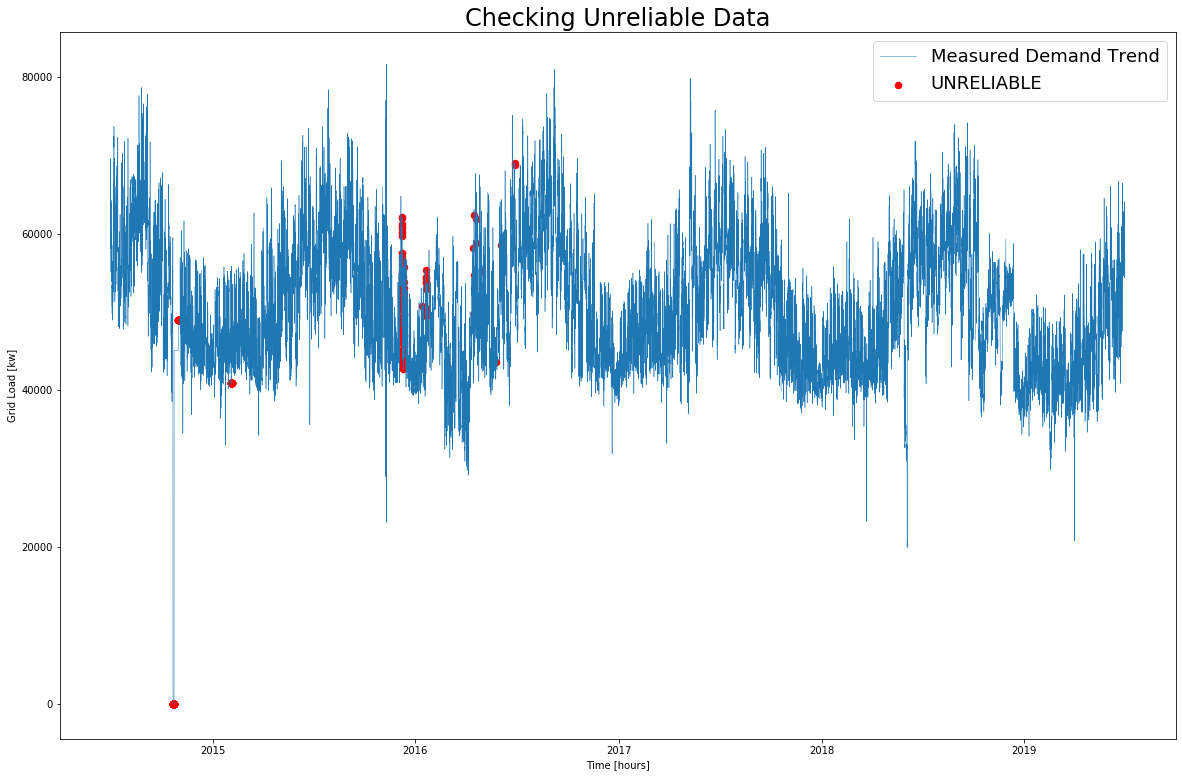
\includegraphics[width=\textwidth]{./figures/unreliable.png}
	  \caption{Some of the campus data has been flagged as unreliable. This usually caused by instrument failure.}
	  \label{fig:unreliable}
	\end{figure}
	This data has been mined and processed to obtain some interesting relationships.
	We've also found some interesting \textit{absent} relationships. Figure \ref{fig:demandfreq} shows two significant peaks in the temperature frequency
	curve, and several significant peaks in the demand frequency curve. These peaks
	indicate \textit{seasonalities} for each set of data. The peaks at 1 and 365
	indicate yearly and daily trends, respectively. However, campus demand exhibits
	trends that temperature does not, such as weekly variation due to low demand
	on weekends. For this reason, the yearly trends for demand and temperature are
	highly correlated, with a Pearson correlation of $r=0.97$, while the daily trends have a much lower correlation of $r=0.69$. Figure \ref{fig:tempcorrelation} shows this correlation and a polynomial characteristic
	function that fits the data. This line give a simple first order relationship
	that allows us to guess a demand based on the temperature. Figure
	\ref{fig:yearlytrends} shows the yearly trends for electricity demand and air
	temperature on campus.

	\begin{figure}[H]
	  \centering
	  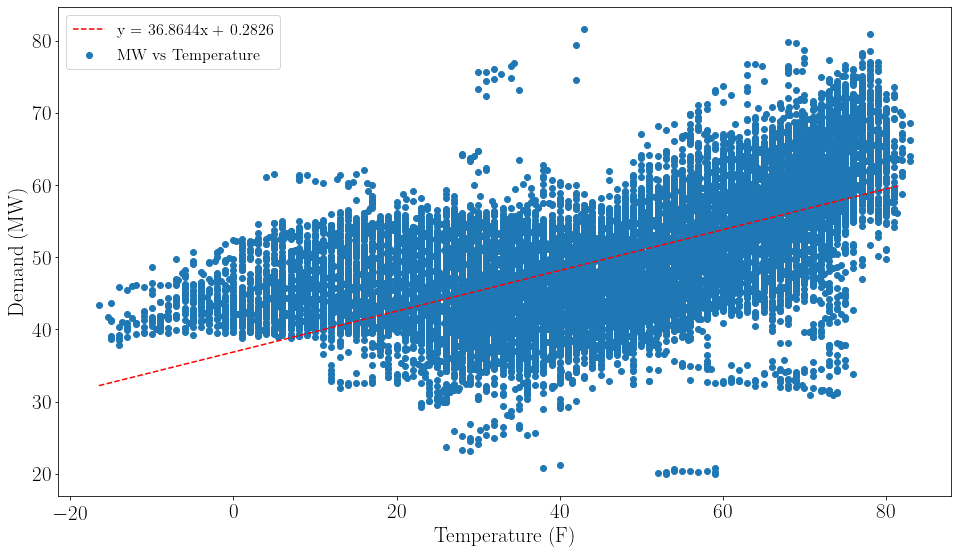
\includegraphics[width=\textwidth]{./figures/demandtempcorr.png}
	  \caption{The correlation and best fit line for campus demand and wet bulb
	  temperature.}
	  \label{fig:tempcorrelation}
	\end{figure}

	The electricity demand below 40$^\circ$F appears to flatten out because energy
	demand on campus switches to steam for district heating. 

	\begin{figure}[H]
	  \centering
	  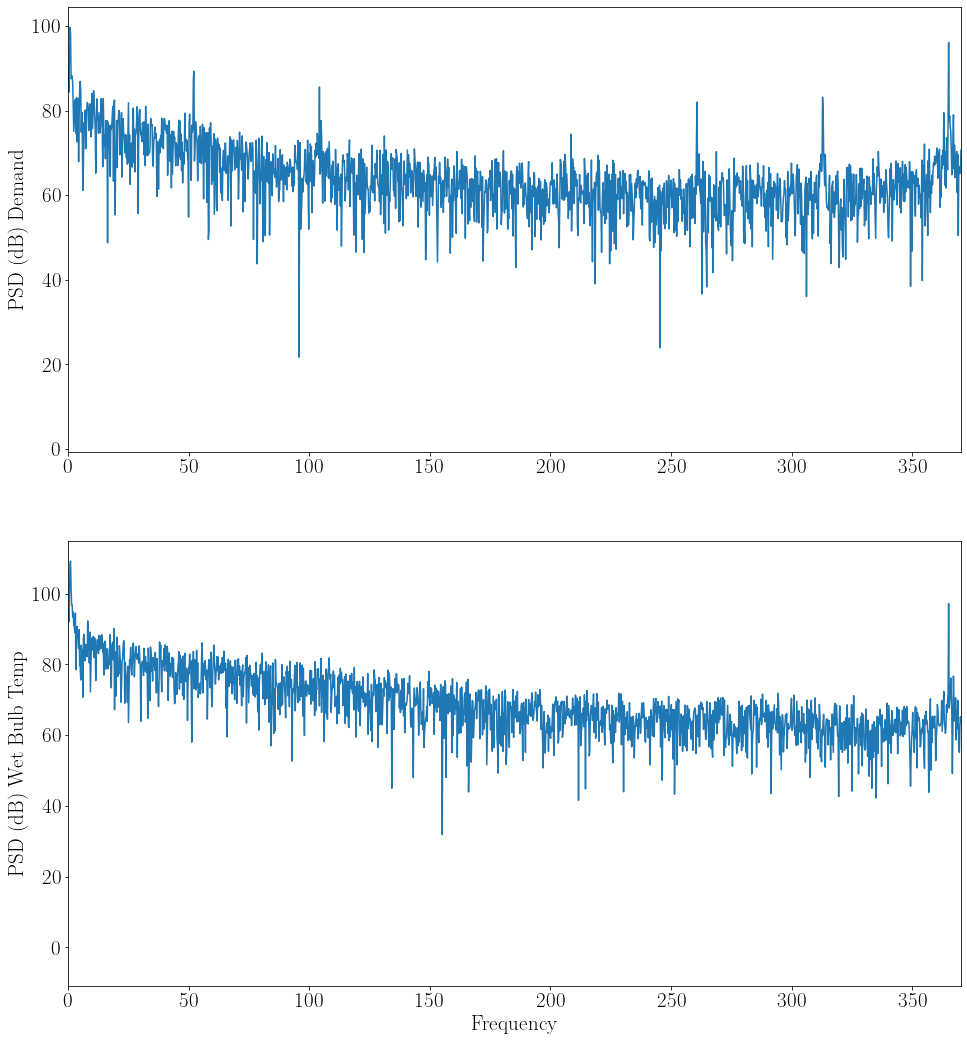
\includegraphics[width=\textwidth]{./figures/demandtempfreq.png}
	  \caption{Show the frequency peaks after taking the Fourier transform of data.}
	  \label{fig:demandfreq}
	\end{figure}

	\begin{figure}[H]
	  \centering
	  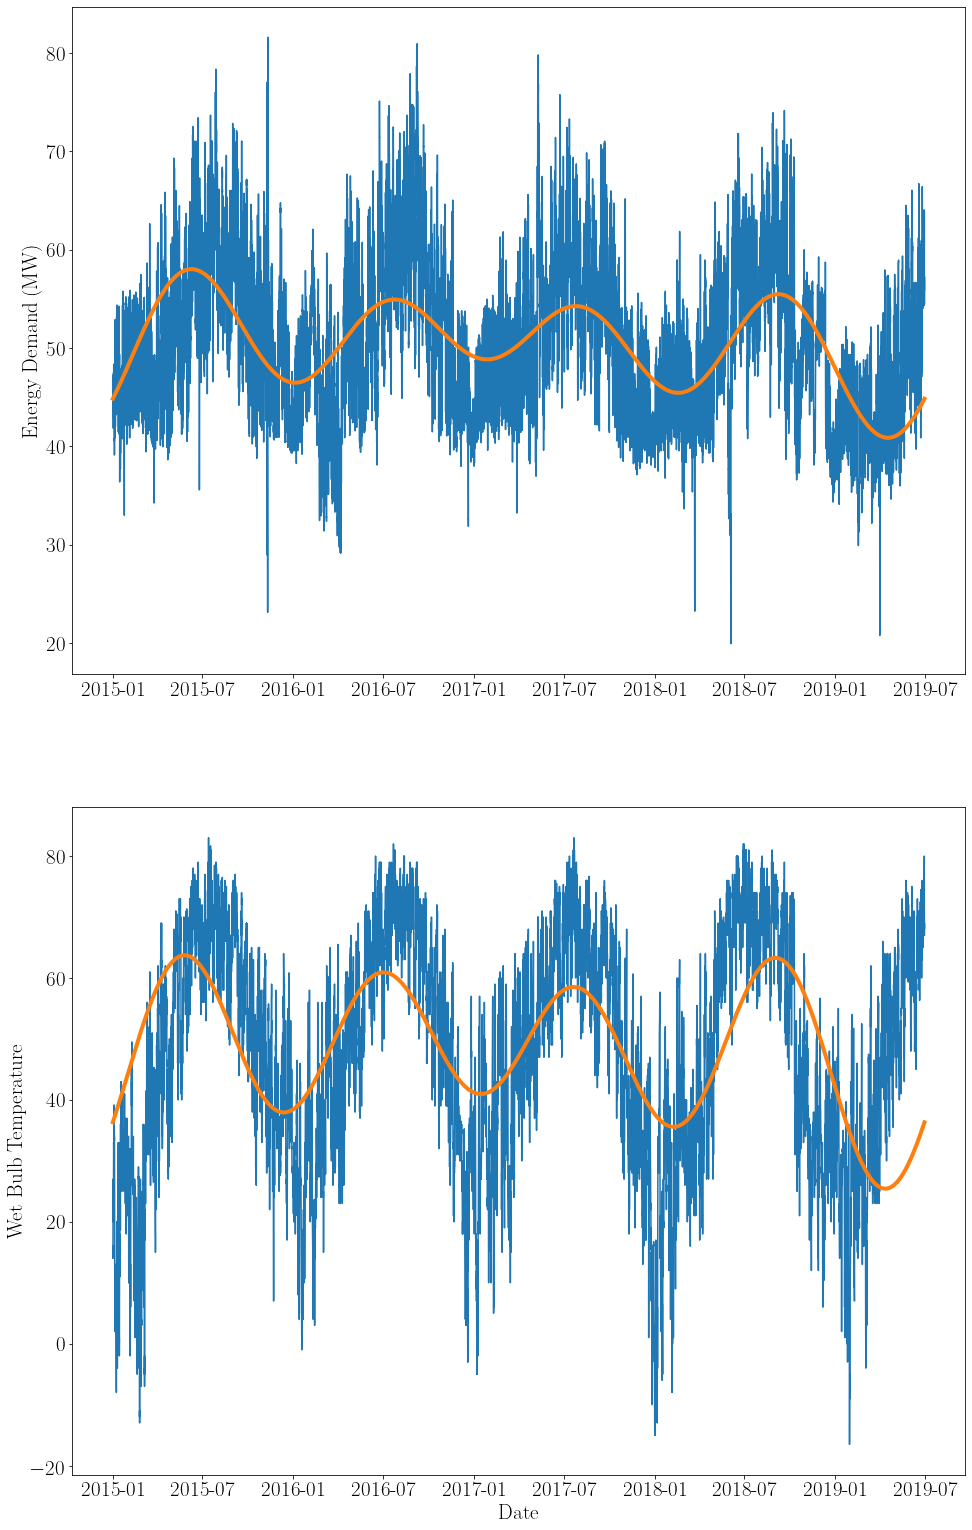
\includegraphics[width=\textwidth]{./figures/yearlytrends.png}
	  \caption{Show the yearly trends for demand and temperature on campus.}
	  \label{fig:yearlytrends}
	\end{figure}



%==============================================================================
%==============================================================================
% BEGIN SUMMARY TABLE
%==============================================================================
%==============================================================================
\begin{landscape}

  \begin{table}
    \centering
    \caption{Summary of Currently Available Data}
    \label{tab:datasummary}
    \begin{tabular}{c|c|c|c|c|c}
      \hline
      Data & Resolution & Span & Supply/Demand & Units & Source\\
      \hline
      Abbott Electricity Generation & Hourly & Fiscal$^{\text{a}}$ Years [2015, 2019]& Supply & kW & UIUC F\&S$^{\text{c}}$\\
      Campus Electricity Demand & Hourly & Fiscal Years [2014, 2019] & Demand & kW & UIUC F\&S \\
      Wind Energy to Campus & Hourly & Fiscal Years [2016, 2019] & Supply & kW & UIUC F\&S \\
      UIUC Solar Farm 1.0 & 15-minute & Calendar Years (2015, 2019] & Supply & kW & AlsoEnergy \cite{alsoenergy_university_2019}\\
      Solar Irradiance & 30-minute & Calendar Years [2013, 2018]& [-] & W/m$^2$& OpenEI \cite{sengupta_national_2018}\\
      Campus Steam Demand & Hourly & Fiscal Years [2015, 2019] & Supply & Klbs & UIUC F\&S\\
      Lincoln Weather Data$^{\text{b}}$ & Hourly & Calendar Years [2010,2019] & [-] & Varied & NOAA \cite{noauthor_climate_nodate} \\
      Champaign Weather Data $^{\text{b}}$& Hourly & Calendar Years [2010,2019]& [-] & Varied & NOAA \cite{noauthor_climate_nodate}\\
      Campus Fuel Demand & Daily & Calendar Year [2019]& Demand & Gallons & UIUC F\&S \\
      Total UIUC Fuel Demand & Yearly & Calendar Year [2019]& Demand & Gallons & UIUC F\&S \\
      CU-MTD Fuel Demand & Daily & Fiscal$^{\text{d}}$ Year [2018]& Demand & Gallons, Dollars & CU-MTD$^{\text{c}}$ \\
      Abbott: Low Pressure Steam & Minute & Calendar Year [2019] & Supply & Klbs & UIUC F\&S\\
      Abbott: High Pressure Steam & Minute & Calendar Year [2019] & Supply & Klbs & UIUC F\&S\\
      Campus Electricity Demand & Minute & Calendar Year [2019] & Demand & kW & UIUC F\&S\\
      Chilled Water System & Minute & Calendar Year [2019] & Supply/Demand & Tons & UIUC F\&S\\
      Thermal Energy Storage & Minute & Calendar Year [2019] & Storage & Tons & UIUC F\&S\\
      UIUC Solar Farm & Minute & Calendar Year [2019] & Supply & kW & UIUC F\&S\\
      UIUC Total Natural Gas & Minute & Calendar Year [2019] & Demand & BTU & UIUC F\&S\\
      Bluewaters Supercomputer & Hourly & Fiscal Years [2014,2018] & Demand & kW & UIUC F\&S\\
    \end{tabular}
    \subcaption{The UIUC fiscal year runs from August 1 to July 31.}
    \subcaption{See Table 2 for further breakdown of weather data.}
    \subcaption{This data is proprietary \textit{unsure about citation}.}
    \subcaption{The CU-MTD fiscal year runs from July 1 to June 30.}
  \end{table}
\end{landscape}

%==============================================================================
%==============================================================================
% BEGIN WEATHER TABLE
%==============================================================================
%==============================================================================

\begin{table}
  \centering
  \caption{Description of available weather data}
  \label{tab:weather}
  \begin{tabular}{c|c}
  \hline
  Variable  & Units\\
  \hline
  Dry Bulb Temp  & $^\circ$F\\
  Wet Bulb Temp  & $^\circ$F\\
  Precipitation  & inches \\
  Relative Humididty  & \%\\
  Wind Direction  & $^\circ$\\
  Wind Speed  & m/s\\
  Station Pressure & in. Hg \\
  \end{tabular}
\end{table}


\bibliographystyle{unsrt}
\bibliography{bibliography}
\end{document}
